\chapter{Chapter A}

\section{A build system for LaTeX}

texmake is a build system for latex projects. 
%
In the early days I built my documents by calling all the commands from the command line.
%
After a while, I got sick of that, and went through a few iterations of a latex makefile, the primary goal being that the document will only build if it had to and it would call latex and bibtex as many times as was necessary. 
%
Then, from collaborating on documents, I started getting annoyed by dealing with all the intermediate files that latex generates that don't really belong in source control. 
%
I began looking at writing a cmake module, but cmake is really organized around the way c code is compiled... and didn't extend as well as I had hoped to latex. 
%
So, I wrote texmake.

Texmake is written in perl, and uses only a couple of standard CPAN modules.

\section{Keeping it simple}

texmake tries to eliminate as much work as possible from the document writer.
%
It will try to figure out and resolve dependencies, including graphics files which require conversion from their source format. 
%
This is particularly useful when the document is under version control, as plain-text svg files can be versioned rather than the generated eps/pdf files. 
%
It also allows for out-of-source builds, so that the source directory doesn't get all cluttered with the intermediate files that latex generates. 
%
Lastly, it simplifies the process of generating multiple output formats from a single set of sources (i.e. (x)html, pdf, eps, epub versions). 

\section{Example}

Consider this scenario: We have a very long complicated report to write (i.e. software manual, end-of-project report, thesis, how-to-book). 
%
We want to generate both a full version, and a simplified quick-start kind of version. 
%
The quick start version will contain a subset of the chapters of the full version. 
%
The quick start will be published in PDF and HTML (i.e. web-friendly). 
%
The long version will probably be a large document and we don't really want it to be browsed on-line, but it is likely to be printed, so we'll put it in pdf and dvi format, as well as epub for people who have e-readers.

\begin{figure}[H]
    \centering
    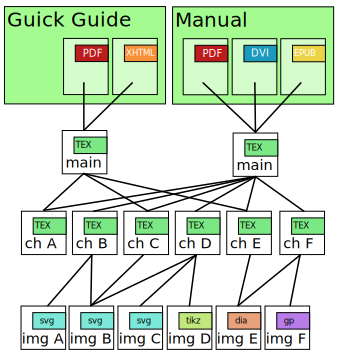
\includegraphics{fig/structure}
    \caption{Source File Structure}
\end{figure}

In the process of making this document, we've generated many image files.
%
Some of them are hand drawn SVGs.
%
Some of them are generated tikz images. 
%
Some of them are diagrams drawn in DIA or plots in GNU Plot. 
%
Some of these figures are shown in multiple different chapters (because the author does not want to just refer the user back to an earlier page, which is unnecessary in an electronic format, but may be more meaningful in a print format).

Furthermore, we have some things that need to only be included in each version. 
%
For instance each version should include some kind of header which tells the reader where he can find the other versions online, or where he can order them from. 
%
Alternatively, perhaps some versions are meant for print and are more conservative with graphics and colors, while an electronic version is a bit more verbose.

Now, we can go maintain a makefile structure that manages all of this quite easily, but we will have to build it by hand. 
%
Every time we add a new chapter or image or output format, we have to go add a line to a makefile somewhere. 
%
Wouldn't it be nice if all of that work would just happen?

\section{The Dependency Graph}

texmake works by building a dependency graph. 
%
When a texmake is first run, it initializes the depency graph by linking the output file to a root source file, which inputs the actual (original) source file.

\begin{figure}[H]
    \centering
    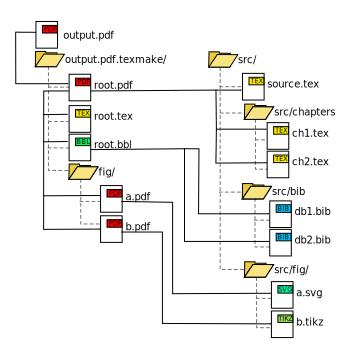
\includegraphics{fig/dependencies}
    \caption{Dependency Graph}
\end{figure}

When texmake is run to make the document, it calls (pdf)latex(ml) to generate the document, and scans the output.
%
If latex can't find a graphics file, it looks a little harder, and tries to find a file with the same basename, and then sees if it knows how to convert it to the format latex might want (i.e. pdf,eps, or png, depending on what the output format is). 
%
If it finds such a file it knows how to convert, it appends the source image and output image to the dependency graph, along with a build rule for generating the output from the input. 
%
The scanner also determines if the document uses bibtex, has a table of contents, or generates aux files.

\section{Features}

here is a list of some of texmake's big features

\begin{itemize}
    \item in single source builds, only generate output documents which use files that have changed
    \item monitor documents dependency on package, style, and class files so that document is rebuilt if these are updated (particularly useful if one is working on a package or style)
    \item only run bibtex if needed
    \begin{itemize}
        \item one of the database files is updated
        \item there are unresolved citations in the document
    \end{itemize}
    \item rerun latex until it stabilizes 
    \begin{itemize}
        \item don't depend on the output of latex to tell us when, since latex doesn't seem to know when table-of-contents entries are out of date
    \end{itemize}
    \item discover and automatically convert graphics source files (like svg) to the kind (pdf)latex(ml) understands (pdf,eps,png)
    \item out of source builds so that sources can be in version control without complicated ignore rules
    \item caches values of environment variables and binary locations so that initial environment does not have to be manually set-up each time the document is built
    \item colorize output to make it clear where and when things get messed up
\end{itemize}


\section{Usage}

texmake relies on the presence of a \verb|texmake.pl| file in the directory of the document you want to build. 
%
The \verb|texmake.pl| file is evaluated by perl, so any perl code can be used, but normally it just calls certain functions that are exposed by the initializer, to add a new target or register a new builder. 
%
Multiple output files can be built from the same input file, so that the same latex source can be used to generate pdf, dvi, and xhtml versions (so-called single source builds). 

\verb|texmake init| is called from the build directory, accepting a single parameter being the directory that contains the root \verb|texmake.pl|. 
%
texmake resolves the absolute path to all the tools it needs (\verb|latex|, \verb|pdflatex|, \verb|bibtex|, \verb|latexml|, ...), and caches those locations. 
%
(TODO: also cache environment variables at time of \verb|init|). 
%
It generates a makefile in that directory which contains rules for all of the output files registered, and creates directories, if they're missing, in which the output files will be located. 

The output files are built with \verb|texmake make|. The texmake builder runs (pdf)latex(ml) with all the necessary switches to make sure that the source directory and output directory are searched for required files. 
%
The builder also scans the output of latex to build a list of all the files that latex loads (for the dependency graph) as well as all the files that are missing. 
%
If the missing files are graphics files, then it generates make rules for how to build those graphics files from similarly named graphics files in the source directory (it is assumed the source file has the same name, but a different extension). 
%
This way, an svg source file can be used to generate pdf,eps,or png images depending on if the document being built is dvi,pdf, or xhtml (respectively). 
%
If the file in the source directory is already compatible with the latex that is being used, then no conversion is necessary. 
%
If the missing file is a bibliography file, then bibtex is run to generate the bibliography file. 
%
The builder also scans the output of bibtex to add bibliography database files (.bib files) to the dependency graph. 
%
Bibtex is also run if there are missing citations reported by latex (this is because bibtex will not include bibliography entries that are not cited in the latex source, so if a new citation is added, bibtex will need to be rerun). 
%
The texmake builder also scans the output of latex for rerun suggestions. 
%
It will rerun latex if it had to run bibtex, or if latex itself suggested that it be rerun (to get cross references straight, for example).




